% Note that if you want something in single space you can go back and
% forth between single space and normal space by the use of \ssp and
% \nsp.  If you want doublespacing you can use \dsp.  \nsp is normally
% 1.5 spacing unless you use the doublespace option (or savepaper
% option)
%
%(FORMAT) usually you *don't* want to mess with the spacing for your
%(FORMAT) final version.  If you think/know that the thesis template
%(FORMAT) and/or thesis style file is incorrect/incomplete, PLEASE
%(FORMAT) contact the maintainer.  THANK YOU!!!

\chapter{BACKGROUND}
\label{chap:intro}
% By labeling the chapter, I can refer to it later using the
% label. (\ref{chap:background}, \pageref{chap:background}) Latex will take care
% of the numbering.

In this research thesis, geometric algorithms are considered primarily in the context of GIS applications. This focus of my research comes in part because I have a few years of experience working in the GIS field. A geographic information science (GIS) integrates hardware, software, and data for capturing, managing, and displaying all forms of geographically referenced information. GIS allow us to view, understand, question, interpret, and visualize data in many ways that reveal relationships, patterns, and trends in the form of maps, globes, reports, and charts. A GIS helps you answer questions and solve problems by looking at your data in a way that is quickly understood and easily shared \cite{esriDef}. Answering these geographic questions is not a trivial task and often requires detailed understanding of the algorithms required to solve these problems. Geometric algorithms are heavily used in this area and are typically included as a geo-processing tool in most of the GIS software.

To give a simple example, consider that Starbucks coffee chain wants to open a new store in the state of California. The company will want to determine the optimum location as a function of numerous variables characterizing the available physical space and the socioeconomic demographics around it. This process, if done manually by a person with expertise, can literally take many days and even weeks to produce a correct answer. This task can be completed in a few minutes with the help of the right geo-processing tools, which internally implement computational geometric algorithms (for example the Voronoi diagram). Some of the variables this tool would take into consideration are the population density, average income, proximity of existing stores, other competing stores, etc. These algorithms must be made as efficient as possible because they typically operate on huge datasets and do many complex calculations for each item.

These are some of the areas in which geometry algorithms play a critical role.  Since everything we see and touch has a geometric aspect enabling us to understand our world, and the computer graphics and geometry ball is on the roll and gaining momentum, more-and-more areas of endeavor will start to be influenced by geometry algorithms.  You will recognize them when you see them.  But, will you know the best algorithms for new areas of application?  Knowing the fundamentals, and the scope of our current knowledge will help.

\section{Algorithms}

The past three decades have seen phenomenal advances in our knowledge about geometry algorithms.  The activity has been so great and so original that one might even consider it to be a long overdue revival.  It is more than just shaking the bones of Greek skeletons in front of us.  The massive nature of the problems involved goes as far beyond the Greeks as they went beyond the Egyptians \cite{SOFTSURFER}.  Some of the most significant achievements are given in a recent (1996) report ``Strategic Directions in Computational Geometry" \cite{STRATEGICDIRCG}. Other notable examples are:

\subsection{Voronoi Diagram}

The partitioning of a plane with n points into convex polygons such that each polygon contains exactly one generating point and every point in a given polygon is closer to its generating point than to any other is known as a Voronoi diagram \cite{Voronoi}. Lots of useful information can be gathered from the Voronoi diagram. For example, if the polygons have common boundary then the sites located in these polygons are likely to be in direct competition for customers which live in those regions. Hot spots where the distance between the sites and the people are greater than a minimum threshold can be easily figured out which can be potential places for new stores to be setup. These types of information can be a lot of help in taking strategic business decisions. Besides these there are other useful applications of the Voronoi diagram. 
\begin{itemize}
\item In mining, Voronoi polygons are used to estimate the reserves of valuable materials, minerals or other resources. Exploratory drill holes are used as the set of points in the Voronoi polygons.
\item In machine learning, Voronoi diagrams are used to do 1-NN classifications \cite{MachineLearning}.
\item Voronoi diagrams are also used to compute the roundness of a set of points.
\end{itemize}

Consider another example where a highly flammable liquid needs to be transported by road from location A to location B. The driver would certainly not use the normal geographical positioning system (GPS) which we use in our cars to find the route. In this special scenario the driver does not care about the shortest route in order to save the gas cost. The driver would try to avoid densely populated city areas and roads with steep slopes. These geographic factors need to be considered so that in case of any accident or spills there would be least casualty and harm to common people. Again a Voronoi diagram could be used, but with a different and likely non-uniform distance metric. Still, other geometric algorithms may be used, depending on the choices made by the software developer about representation of relevant information and so on. Solving this can be done in a few minutes or possibly even seconds using a good geo-processing tool. Such a tool can use existing files about geographic information from the area to help the developer even decide on those representation issues and other constraints that permit the modeling of this problem.

\subsection{Polygon Triangulation}

Triangulation or Polygon Triangulation is a fundamental problem in computational geometry, because the first step in working with complicated geometric objects is to break them into simple geometric objects. The simplest geometric objects in a two dimensional space is a triangle. Classical applications of triangulation include finite element analysis and computer graphics. A particularly interesting application of triangulation is surface or function interpolation. Suppose that we have sampled the height of a mountain at a certain number of points. How can we estimate the height at any point (Q) in the plane? If we project the points on the plane, and then triangulate them, the triangulation completely partitions the plane into regions. We can estimate the height of Q by interpolating among the three points of the triangle that contains it. Further, this triangulation and the associated height values define a surface of the mountain suitable for graphics rendering. 

Another important and useful application is to strategically place security cameras in order to guard a restricted place. These cameras are usually hung from the ceiling and it is important to place the cameras at strategic locations so that it covers all the regions and at the same time have minimum number of cameras in order to minimize the cost. This problem can be easily solved using polygon triangulation algorithm. A camera position in the gallery corresponds to a point in the polygon. A camera sees those points in the polygon to which it can be connected with an open segment that lies in the interior of the polygon.

\subsection{Point Location}

Point Location is another hot topic and algorithm which is now-a-days famous. This algorithm basically tries to find the location of point in the space. In simple terms this means to find the query point in a plane which could be comprised of several disjoint regions. Point location queries arise in various settings. The simplest and most common example is to find the current location while driving a car using a global positioning system (GPS). Another application in terms of computer systems is to find the region where the user clicked using the mouse button. The task here is to find the region on the screen where the user clicked the mouse button which could be a button, image, list box or simply nothing but desktop.

\subsection{Delaunay Triangulation}

A Delaunay Triangulation for a set P of points in a plane is a triangulation DT(P) such that no point in P is inside the circumcircle of any triangle in DT(P). Delaunay triangulations maximize the minimum angle of all the angles of the triangles in the triangulation; they tend to avoid skinny triangles. The triangulation is named after Boris Delaunay for his work on this topic from 1934. \cite{Delanuay, SOFTSURFER, DelanuayWiki}
\begin{itemize}
\item The Euclidean minimum spanning tree \cite{SpannigTree} of a set of points is a subset of the Delaunay triangulation of the same points, and this can be exploited to compute it efficiently. 
\item For modeling terrain or other objects given a set of sample points, the Delaunay triangulation gives a nice set of triangles to use as polygons in the model. In particular, the Delaunay triangulation avoids narrow triangles (as they have large circumcircles compared to their area).
\item Delaunay triangulations can be used to determine the density or intensity of points samplings by means of the DTFE. \cite{DTFE}
\item Delaunay triangulations are often used to build meshes for space-discretized solvers such as the finite element method and the finite volume method of physics simulation, because of the angle guarantee and because fast triangulation algorithms have been developed. Typically, the domain to be meshed is specified as a coarse simplified complex; for the mesh to be numerically stable, it must be refined, for instance by using Ruppert's algorithm. \cite{RuppertAlgo}
\end{itemize}

\section{Maps and Geographic Information Science (GIS)}

Maps are an invaluable source of information and are used in many day to day activities. Maps have been used since olden days, although maps in those days were not accurate and not scaled properly. But since the last century, mankind has realized the importance of maps and learned proper means of creating and using them; today�s maps are often derived from very precise satellite information. If a map is not constructed properly then it can definitely be a source of frustration. But now-a-days maps are really easy to understand and interpret. Thanks to the vast area of study in geography and evolution of new technology. In today�s world we have digital maps that are really easy to interact with and reveal a wealth of information. A geographic information system splits maps into several layers that are super imposed upon each other and thus present a map that is really a stack of layers drawn on top of one another. For example, consider a map showing the vegetation in the state of California. Initially there would be a layer drawing the map of the state of California and then there would be second layer showing the vegetation that would be drawn on top of the layer of California. The first layer is usually called as a Basemap Layer. It is very important that all the layers in map are in sync with each other.  In GIS terms this is referred to as a spatial reference. Spatial reference is the coordinate system, tolerance, and resolution used to store the spatial dataset. In other words consider spatial reference as the reference point with respect to with, each layer is drawn. In a digital map the visibility of any layer can be turned off easily by the click of a mouse button thus giving the user the power to hide/ unhide any information at any particular instance of time. 

Having given some preliminary description about computational geometry, its algorithms, geographic information science (GIS) and maps we will now turn our attention to the contribution of this thesis research.  This thesis research is about a particular type of spatial algorithm which is commonly known as a Line Sweep Algorithm or Plane Sweep Algorithm. There are many algorithms that use the line-sweep technique. One algorithm in particular tries to find intersections among line segments belonging to two different sets in a two dimensional co-ordinate system. The problem of finding and reporting all pair-wise intersections in a set of line segments is among the first to have been studied in computational geometry; its solution established the use of sweep-line methods and introduced the notion of output sensitive algorithms. In the early days of computational geometry, Bentley and Ottmann \cite{BentleyOttmann} introduced their well-known line sweep algorithm. Mairson and Stol \cite{Stol} were the first to find an asymptotically optimal algorithm running in {\it O}(n log n + k) time.

Consider that a city planner wants to find out the location where there is a need to build bridges. The city planner would first prepare a map of the city. This data is generally freely available on most government and educational websites. Then the planner would put a layer of rivers flowing through the city and finally he/she would put a layer of roads in the city on top of the rivers (Figure.~\ref{fig2} \cite{MAP}). Now the answer to the question of the places where bridges need to be built is basically the places where roads and rivers intersect. The line sweep algorithm can be useful in finding the solution to this question. The rivers are generally not straight and are curvy. These curved lines can be represented by a collection of many small adjacent segments. Then one set of line segments can represent the rivers flowing through the city and the second set of line segments can represent the roads in the city. Now we need to find out intersections among these line segments, which might be appropriate candidates for places where bridges need to be built. This algorithm to find intersections among set of line segments seems trivial. But this is a complex algorithm and must be highly efficient, especially given the potentially large number of segments involved in a real world situation as described. Imagine running this algorithm on tera-bytes of a raster image and finding out the correct result in a matter of few seconds.
\begin{figure}[ht]
  \begin{center}
   	\fbox{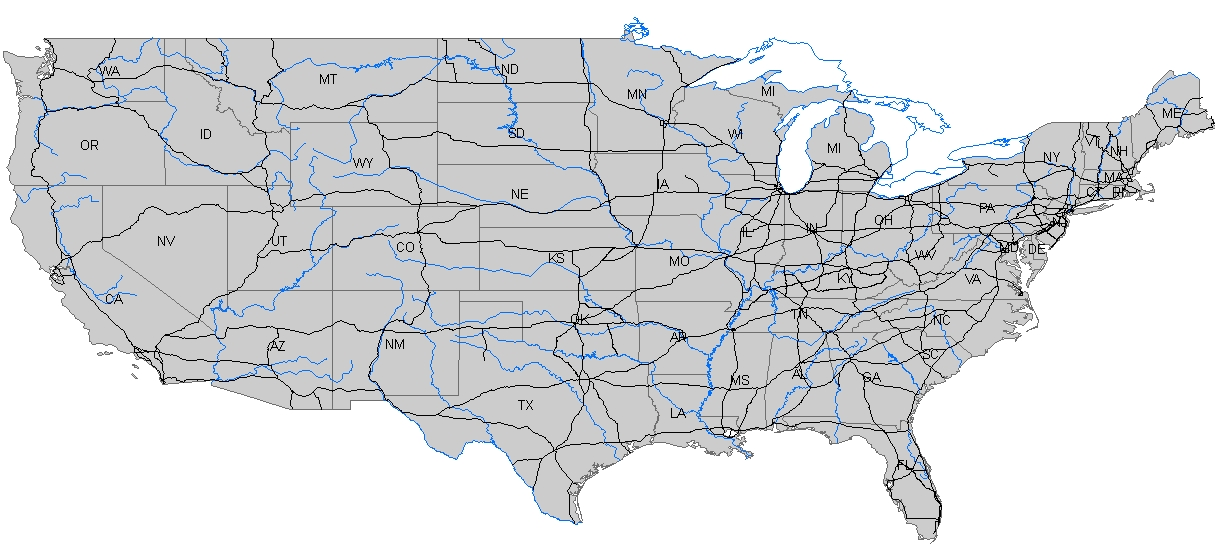
\includegraphics[width=4.5in]{Figures/Figure2}}
  \end{center}
  \centering
	\parbox{4.5in}{\caption{Map of USA showing roads and rivers. Source: ESRI, \textbf{\textit{Arcgis online}}. ArcGIS, http://www.arcgis.com, accessed Aug. 2012, n.d.} \label{fig2}} 
\end{figure}

Other algorithms that typically use the line sweep technique are Voronoi diagrams, finding nearest object, triangulation, two-dimensional and three-dimensional point location, shortest path and many others in GIS as well as in other fields.

I was once asked a question during an interview; it was amazing how easily I could relate the question to this algorithm and present a solution. I was given a scenario where there is a multinational company that has three phone servers. People could make calls at any time during the day. I was asked to propose an algorithm that would determine the peak time during the day when most calls were made. I thought for about 5-10 minutes and suddenly it struck my mind that this problem can be solved using the line sweep algorithm. Imagine a two dimensional space for each server where x-axis is represented by the duration of phone call and y-axis is represented by the time in a day. Then we would get several lines representing the calls made during that day for each server as horizontal lines in the XY co-ordinate space. Now image a horizontal line sweeping this graph from top to bottom. Each time it would intersect the calls made during the day, we would record the total number of intersections intersection. When the imaginary line sweeps the graph completely then we would have the answer for the peak time when maximum calls were made during the day.

Like this example, there are many other scenarios where a line sweep algorithm might be useful, which makes me appreciate this algorithmic technique even more. I studied this algorithm and thought of altering one of the data structure used by it. The goal of the alteration would be to enhance the efficiency of this algorithm by modifying one of the data structure used by line-sweep algorithm, namely status structure such as in the line-segment intersection problem, is the objective of this research. The status structure is used to keep track of the segments currently adjacent to one another and the proposed alteration will increase the efficiency of search operations on this structure.

\section{Supporting Research}
Several other people have worked and been working on various aspect of this algorithm. Many of them have published papers regarding their work. It is quite interesting to see so much work going around in this work on this algorithm. Notable among the published papers are ``Feature Analysis Using Line Sweep Thinning Algorithm" \cite{FeatureAccessThinningAlgo} and ``A Sweep line approach to Interconnect Testing" \cite{InterconnectTesting}.
